\documentclass[glossy]{beamer}
\useoutertheme{wuerzburg}
\useinnertheme[realshadow,corners=2pt,padding=2pt]{chamfered}
\usecolortheme{shark}

\usepackage{listings}
\usepackage[utf8]{inputenc}

\usepackage{tikz}
\newcommand<>{\hover}[1]{\uncover#2{%
 \begin{tikzpicture}[remember picture,overlay]%
 \draw[fill,opacity=0.4] (current page.south west)
 rectangle (current page.north east);
 \node at (current page.center) {#1};
 \end{tikzpicture}}
}

\title{Concurso PAD - Área Arquitectura de Computadoras\\\line(1,0){320}}
% \author{\texorpdfstring{Author\newline\url{email@email.com}}{Author}}
%\author{Rafael Ignacio Zurita}
\institute{Rafael Ignacio Zurita \\ Departamento de Ingenieria de Computadoras \\ Clase de oposición}
%\date{\today}



\begin{document}




\begin{frame}
\maketitle
\end{frame}

\institute{Rafael Zurita - Departamento de Ingenieria de Computadoras - FAI - UNCOMA \\ 2018}

\begin{frame}
\frametitle{Programa Analítico}
	\begin{center}
\textbf{Jerarqu\'ia de Memoria}
	\end{center}
\begin{itemize}
\item Computador actual y renovación (que comprar)
\item Los programadores quisieron siempre ilimitada cantidad de memoria
\item tendencia de las ultimas decadas en el diseño tecnológico de CPU y memoria principal
\begin{itemize}
\item Las cpu se diseñaron con mejor performance, las memorias principales (DRAM) se diseñaron con el objetivo de ser mas densas y baratas, luego performance
\end{itemize}
\item Tecnología actual ya vista (UNIDAD II) flip-flops D para registros y memoria statica
\item Idea clave: tener los datos correctos, en el lugar preciso, en el momento adecuado
\begin{itemize}
\item Y que significa lo anterior: analogia del alumno y el examen (papel, lapiz, calculadora)
\end{itemize}

\item Principio de localidad
\item Jerarqu\'ia de memoria: ilimitada cantidad de la memoria más rápida al menor costo
\end{itemize}
\end{frame}

\begin{frame}
\frametitle{Jerarqu\'ia de Memoria}
\textbf{UNIDAD 3: Memoria}

Características de las diferentes tecnologías de memoria. Comportamiento de los programas: principio de localidad. \textbf{Jerarqu\'ia de memoria}. Memoria Cache. Memoria virtual.  

\end{frame}




%
%
%  0.4 cm die = 4mm  16mm^2
%  4mm^2 cache
%  4MB cache
%  400MB 400M^2
%  4GB   4000mm^2
%  16GB  16000mm^2
%   125mm^2  1 metro










\begin{frame}
\frametitle{Jerarqu\'ia de Memoria}
        \begin{center}
        \textbf{Cuando se quiere comprar una computadora nueva...}
        \end{center}
Si ya contamos con una PC CPU core i3 2.6Ghz, 8GB RAM, 512GB disco, \textbf{¿Qué computadora queremos adquirir?:}
\begin{tabular}{cl}

\begin{tabular}{c}
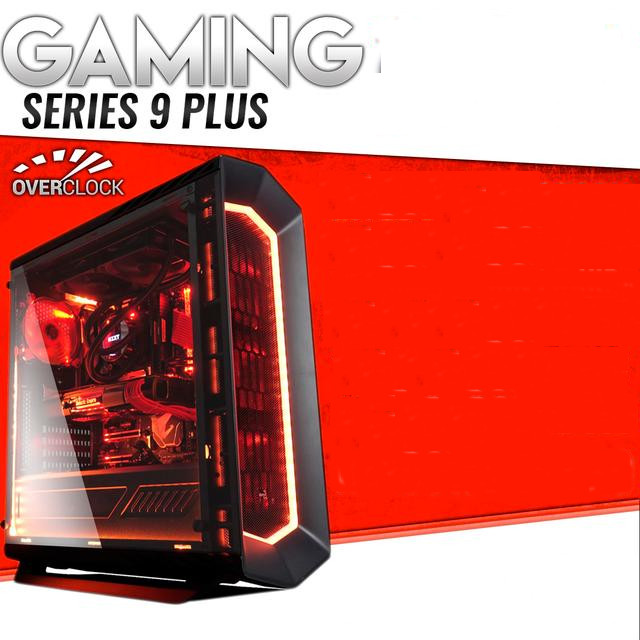
\includegraphics[height=6cm, width=4cm]{pc5.jpg} 

\end{tabular}
& \begin{tabular}{l}
\parbox{0.5\linewidth}{
        \textbf{Procesador}: ..................... \\
        \textbf{Memoria}: ..................... \\
        \textbf{Disco}: ..................... 
}
\end{tabular} \\

\end{tabular}
\end{frame}




\begin{frame}
\frametitle{Jerarqu\'ia de Memoria}
        \begin{center}
        \textbf{Cuando se quiere comprar una computadora nueva...}
        \end{center}
Si ya contamos con una PC CPU core i3 2.6Ghz, 8GB RAM, 512GB disco, \textbf{¿Qué computadora queremos adquirir?:}
\begin{tabular}{cl}

\begin{tabular}{c}
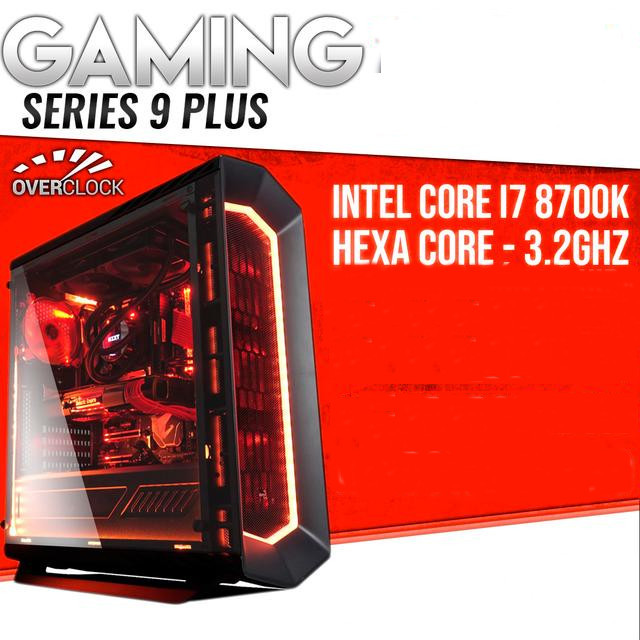
\includegraphics[height=6cm, width=4cm]{pc45.jpg} 

\end{tabular}
& \begin{tabular}{l}
\parbox{0.5\linewidth}{
        \textbf{Procesador}: más rápido, mas cores \\
        \textbf{Memoria}: ..................... \\
        \textbf{Disco}: ..................... 
}
\end{tabular} \\

\end{tabular}
\end{frame}



\begin{frame}
\frametitle{Jerarqu\'ia de Memoria}
        \begin{center}
        \textbf{Cuando se quiere comprar una computadora nueva...}
        \end{center}
Si ya contamos con una PC CPU core i3 2.6Ghz, 8GB RAM, 512GB disco, \textbf{¿Qué computadora queremos adquirir?:}
\begin{tabular}{cl}

\begin{tabular}{c}
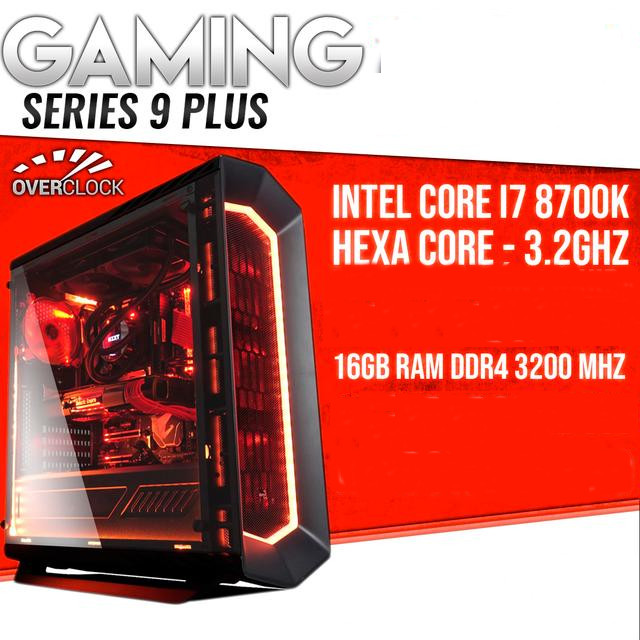
\includegraphics[height=6cm, width=4cm]{pc4.jpg} 

\end{tabular}
& \begin{tabular}{l}
\parbox{0.5\linewidth}{
        \textbf{Procesador}: más rápido, mas cores \\
        \textbf{Memoria}: más memoria \\
        \textbf{Disco}: ..................... 
}
\end{tabular} \\

\end{tabular}
\end{frame}



\begin{frame}
\frametitle{Jerarqu\'ia de Memoria}
        \begin{center}
        \textbf{Cuando se quiere comprar una computadora nueva...}
        \end{center}
Si ya contamos con una PC CPU core i3 2.6Ghz, 8GB RAM, 512GB disco, \textbf{¿Qué computadora queremos adquirir?:}
\begin{tabular}{cl}

\begin{tabular}{c}
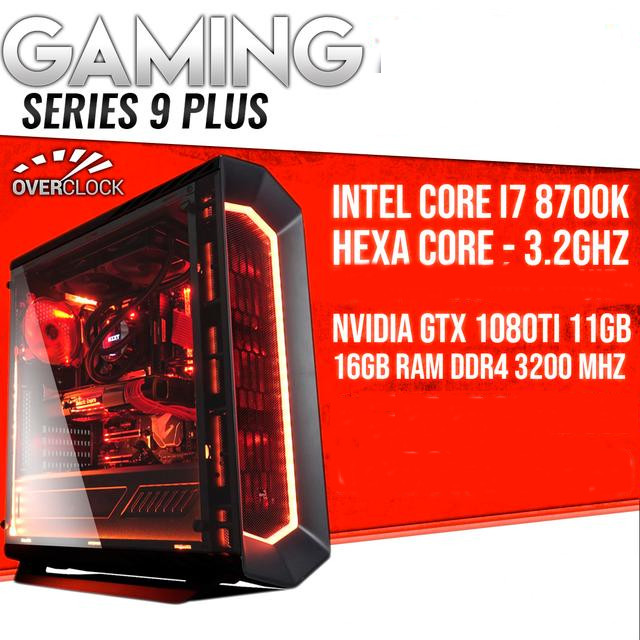
\includegraphics[height=6cm, width=4cm]{pc3.jpg} 

\end{tabular}
& \begin{tabular}{l}
\parbox{0.5\linewidth}{
        \textbf{Procesador}: más rápido, mas cores \\
        \textbf{Memoria}: más memoria \\
        \textbf{Disco}: ..................... 
}
\end{tabular} \\

\end{tabular}
\end{frame}






\begin{frame}
\frametitle{Jerarqu\'ia de Memoria}
        \begin{center}
        \textbf{Cuando se quiere comprar una computadora nueva...}
        \end{center}
Si ya contamos con una PC CPU core i3 2.6Ghz, 8GB RAM, 512GB disco, \textbf{¿Qué computadora queremos adquirir?:}
\begin{tabular}{cl}

\begin{tabular}{c}
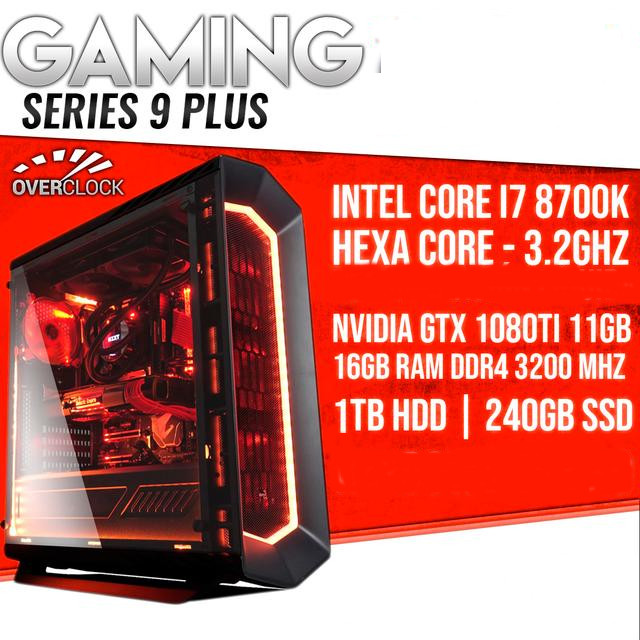
\includegraphics[height=6cm, width=4cm]{pc2.jpg} 

\end{tabular}
& \begin{tabular}{l}
\parbox{0.5\linewidth}{
        \textbf{Procesador}: más rápido, mas cores \\
        \textbf{Memoria}: más memoria \\
        \textbf{Disco}: más disco 
}
\end{tabular} \\

\end{tabular}
\end{frame}






\begin{frame}
\frametitle{Jerarqu\'ia de Memoria}
        \begin{center}
        \textbf{Cuando se quiere comprar una computadora nueva...}
        \end{center}
Si ya contamos con una PC CPU core i3 2.6Ghz, 8GB RAM, 512GB disco, \textbf{¿Qué computadora queremos adquirir?:}


\begin{tabular}{cl}
\begin{tabular}{c}
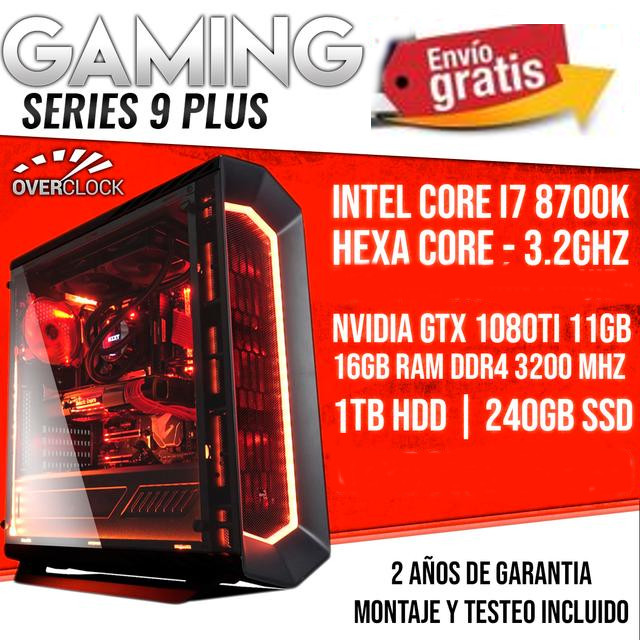
\includegraphics[height=6cm, width=4cm]{pc.jpg} 

\end{tabular}
& \begin{tabular}{l}
\parbox{0.5\linewidth}{
        \textbf{Procesador}: más rápido, mas cores \\
        \textbf{Memoria}: más memoria \\
        \textbf{Disco}: más disco 
}
\end{tabular} \\
\end{tabular}

\end{frame}



\begin{frame}
\frametitle{Jerarqu\'ia de Memoria}
        \begin{center}
        \textbf\textit{"Procesador más rápido, mas cores"}
        \end{center}
\begin{itemize}
\item \textbf{IMPORTANTE}: es tiempo de utilizar mayor precisión y terminología
\item \texit{Ejemplo: "Microprocesador con un rendimiento mayor que el anterior"} 
\begin{itemize}
\item (Es más adecuado)
\item Buscamos que realice una mayor cantidad de trabajo en el mismo tiempo o,
\item la misma cantidad de trabajo que antes, pero en un tiempo menor. 
\end{itemize}
\end{itemize}
\end{frame}






\begin{frame}
\frametitle{Jerarqu\'ia de Memoria}
        \begin{center}
        \textbf{The Memory Wall}
        \end{center}

Año tras año ...
\begin{itemize}
\item Los microprocesadores nuevos son más rápidos (mejoran el rendimiento). 
\item Las memorias nuevas son más rápidas (mejoran el rendimiento).
\end{itemize}

% \begin{itemize}
% \item Pero, año tras año, el progreso en la tecnología de las CPU es mucho mejor que el de las memorias.
% \end{itemize}

% \begin{itemize}
% \item Desde 1986 hasta el 2005 la velocidad de los microprocesadores aumentaba un 55% cada año, mientras que la memoria mejoraba sólo un 10% la velocidad
% \item Llegará el momento en que la memoria será un muro, en donde el progreso de la tecnología de la CPU no tendrá sentido si no existen mejoras tecnológicas en las memorias.
% \end{itemize}

\begin{center}
\begin{figure}
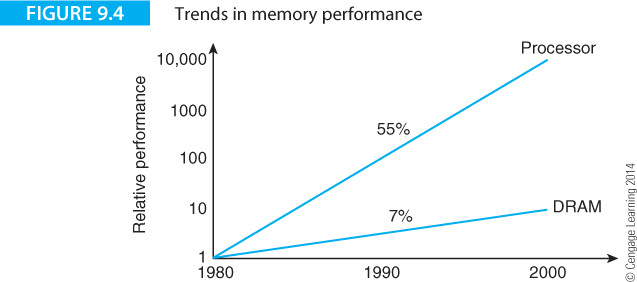
\includegraphics[scale=0.4]{memorywall.jpg} 
\end{figure}
\end{center}
\end{frame}


\begin{frame}
\frametitle{Jerarqu\'ia de Memoria}
        \begin{center}
        \textbf{Memorias}
        \end{center}
\begin{itemize}
\item En una computadora de propósito general se cuenta con:
\begin{itemize}
\item Memoria con Firmware de arranque
\item Memoria RAM (volatil, estática y dinámica/DRAM y caché)
\item Disco rígido o memoria flash
\item Disco de estado sólido
\item DVD y CD
\item Memorias SD y pendrives
\end{itemize}
\end{itemize}

 \textbf{¿Por qué necesitamos tantos tipos de memoria?}
\end{frame}


\begin{frame}
\frametitle{Jerarqu\'ia de Memoria}
        \begin{center}
        \textbf{Memorias}
        \end{center}
\begin{itemize}
\item En una computadora de propósito general se cuenta con:
\begin{itemize}
\item Memoria con Firmware de arranque
\item Memoria RAM (volatil, estática y dinámica/DRAM y caché)
\item Disco rígido o memoria flash
\item Disco de estado sólido
\item DVD y CD
\item Memorias SD y pendrives
\end{itemize}
\end{itemize}

 \textbf{¿Por qué necesitamos tantos tipos de memoria?}
\begin{itemize}
\item Memoria ideal: ilimitada (siempre suficiente), veloz, densa (tamaño físico), de bajo consumo, robusta, barata, persistente. Pero, la tecnología es insuficiente.
\end{itemize}
\end{frame}




\begin{frame}
\frametitle{Jerarqu\'ia de Memoria}
        \begin{center}
        \textbf{Memorias}
        \end{center}
 \textbf{¿Por qué necesitamos tantos tipos de memoria?}
\begin{itemize}
\item Memoria ideal: ilimitada (siempre suficiente), veloz, densa (tamaño físico), de bajo consumo, robusta, barata, persistente. Pero, la tecnología es insuficiente.
\end{itemize}

\begin{center}
\begin{figure}
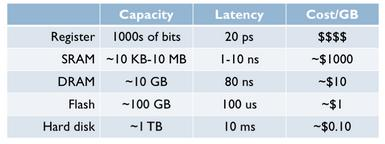
\includegraphics[scale=0.6]{tecnologias.jpg} 
\end{figure}
\end{center}
\end{frame}


\begin{frame}
\frametitle{Jerarqu\'ia de Memoria}
        \begin{center}
        \textbf{Memorias}
        \end{center}
 \textbf{¿Por qué necesitamos tantos tipos de memoria?}
\begin{itemize}
\item Memoria ideal: ilimitada (siempre suficiente), veloz, densa (tamaño físico), de bajo consumo, robusta, barata, persistente. Pero, la tecnología es insuficiente.
\end{itemize}

\begin{center}
\begin{figure}
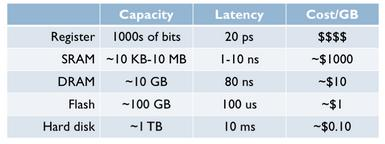
\includegraphics[scale=0.5]{tecnologias.jpg} 
\end{figure}
\end{center}
\begin{itemize}
\item \textbf{IDEA 1}: Exponer todos los tipos de memoria y que el programador la utilice con el mejor rendimiento posible.
\end{itemize}
\end{frame}





\begin{frame}
\frametitle{Jerarqu\'ia de Memoria}
        \begin{center}
        \textbf{Localidad de las Referencias}
        \end{center}
\begin{itemize}
\item \textbf{IDEA 2}: mantener los datos más frecuentemente utilizados por el procesador en una pequeña memoria veloz SRAM (cercana a la CPU) de manera transparente.
\item Hacer referencia a la memoria principal unicamente de vez en cuando.
\begin{itemize}
\item Esta idea libera al programador
\item ¿Qué hace posible esta idea?
\end{itemize}
\end{itemize}

\end{frame}




\begin{frame}
\frametitle{Jerarqu\'ia de Memoria}
        \begin{center}
        \textbf{Localidad de las Referencias}
        \end{center}
\begin{itemize}
\item \textbf{IDEA 2}: mantener los datos más frecuentemente utilizados por el procesador en una pequeña pero veloz memoria SRAM (cercana a la CPU) de manera transparente.
\item Hacer referencia a la memoria principal unicamente de vez en cuando.
\begin{itemize}
\item Esta idea libera al programador
\item ¿Qué hace posible esta idea?
\end{itemize}
\end{itemize}
\begin{itemize}
\item \textbf{Comportamiento de los programas}: si se observa un intervalo corto de tiempo se utiliza una pequeña fracción del total de la memoria.
\item Este comportamiento de acceso ha sido llamado principio de localidad de las referencias[DENN68], o simplemente \textbf{principio de localidad}.
\end{itemize}

\end{frame}







\begin{frame}
\frametitle{Jerarqu\'ia de Memoria}
        \begin{center}
        \textbf{Localidad de las Referencias}
        \end{center}

\begin{tabular}{cl}
\begin{tabular}{c}
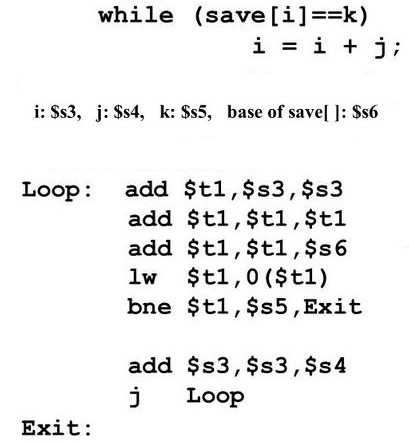
\includegraphics[height=6cm, width=5cm]{ciclo2.jpg} 

\end{tabular}
& \begin{tabular}{l}
\parbox{0.5\linewidth}{
        Repaso de IC: Ciclo de instrucción \\
\\
        El procesador ejecuta las mismas instrucciones varias veces, \\ 
\\
\\
        y tambien accede a elementos del vector save[].
}
\end{tabular} \\
\end{tabular}

\end{frame}





\begin{frame}
\frametitle{Jerarqu\'ia de Memoria}
        \begin{center}
        \textbf{Localidad de las Referencias}
        \end{center}

\begin{tabular}{cl}
\begin{tabular}{c}
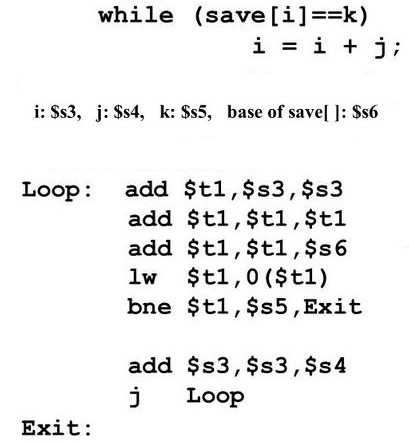
\includegraphics[height=6cm, width=5cm]{ciclo2.jpg} 

\end{tabular}
& \begin{tabular}{l}
\parbox{0.5\linewidth}{
        Repaso de IC: Ciclo de instrucción \\
\\
        El procesador ejecuta las mismas instrucciones varias veces (\textbf{localidad temporal}), \\ 
\\
        y tambien accede a elementos del vector save[] (\textbf{localidad espacial}).
}
\end{tabular} \\
\end{tabular}

\end{frame}



\begin{frame}
\frametitle{Jerarqu\'ia de Memoria}
        \begin{center}
        \textbf{Resumen}
        \end{center}

\begin{itemize}
\item \textbf{Jerarqu\'ia de Memoria}: Organización de la memoria de una computadora que permita 
\begin{itemize}
\item obtener el \textbf{rendimiento} de una memoria de alta velocidad 
\item al \textbf{costo} (precio) de una memoria grande y lenta.
\end{itemize}
\item Idea clave: tener los datos correctos, en el lugar preciso, en el momento adecuado (principio de localidad)
\end{itemize}

\end{frame}




\begin{frame}
\frametitle{Jerarqu\'ia de Memoria}
        \begin{center}
        \textbf{Jerarqu\'ia de Memoria}
        \end{center}

\begin{tabular}{cl}
\begin{tabular}{c}
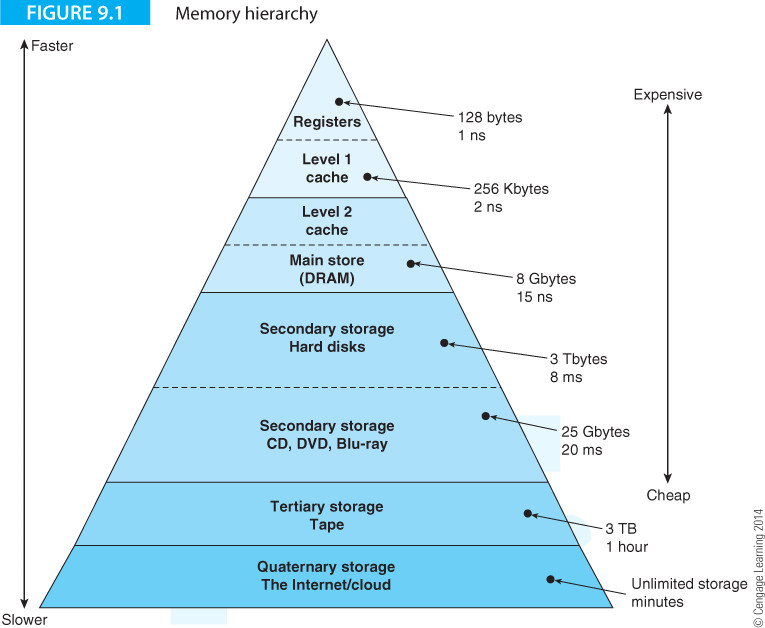
\includegraphics[height=7cm, width=6cm]{jerarquia.jpg} 

\end{tabular}
& \begin{tabular}{l}
\parbox{0.4\linewidth}{
        \footnotesize{Organizar el sistema de memoria dentro de una \textbf{jerarquía de niveles}.} \\
\\
	Cada nivel está compuesto por un tipo de memoria (tecnología) \\
\\
        \textbf{Objetivo}: \textit{obtener el rendimiento de una memoria de gran velocidad al coste de una memoria de baja velocidad, y de tamaño casi ilimitado.}
}
\end{tabular} \\
\end{tabular}

\end{frame}




\begin{frame}
\frametitle{Jerarqu\'ia de Memoria}
        \begin{center}
        \textbf{DRAM vs SRAM}
        \end{center}
\begin{itemize}
\item Factores: densidad, costos, consumo, rendimiento. 
\item ¿Densidad en cachés?
\end{itemize}
\begin{center}
\begin{figure}
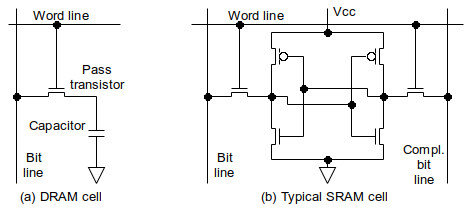
\includegraphics[scale=0.6]{sramvsdram.jpg} 
\caption{DRAM vs SRAM}
\label{DRAM vs SRAM}
\end{figure}
\end{center}
\end{frame}



\begin{frame}
\frametitle{Jerarqu\'ia de Memoria}
        \begin{center}
        \textbf{Resumen}
        \end{center}
Organizando las tecnologías de memoria dentro de una \textbf{jerarquía de niveles}
se puede construir un sistema de memoria de
\begin{itemize}
\item bajo costo y
\item con un rendimiento similar al de una memoria cara y de alta velocidad
\end{itemize}
\\ Si este sistema es transparente al programador
\begin{itemize}
\item ¿Para qué interesa su estudio?
\end{itemize}
\end{frame}


\begin{frame}
\frametitle{Jerarqu\'ia de Memoria}
\begin{center}
\begin{itemize}
\item  ¿Preguntas?
\end{itemize}
\end{center}
\end{frame}





\begin{frame}
 \frametitle{Bibliografía}
        \begin{center}
        \textbf{Material complementario de estudio}
        \end{center}
Apunte de cátedra
\begin{itemize}
\item \textbf{Memoria}, Rafael Ignacio Zurita 2017 (disponible en PEDCO). Versión en español ampliada (con permiso escrito de Prof. Alan Clements y Prof. Hank Levy) de los libros:
\begin{itemize}
\begin{itemize}
\item Computer Organization and Architecture: Themes and Variations, Alan Clements, Cengage Learning, 2013, ISBN: 1285415426, 9781285415420
\item Computer Programming and Architecture the VAX-11, Henry Levy, Digital Press 1980
\end{itemize}
\end{itemize}
\end{itemize}
Libros
\begin{itemize}
\item Andrew S. Tanenbaum (2000), ORGANIZACIÓN DE COMPUTADORAS un enfoque estructurado, Editorial Prentice Hall. (10 copias en biblioteca)
\item David. Patterson John L. Hennessy (1995), ORGANIZACIÓN Y DISEÑO DE COMPUTADORES La interfaz hardware/software, McGraw-Hill (8 copias en biblioteca).
\end{itemize}

\end{frame}


\end{document}
